\documentclass[color,subfigure,epsf,here,cite,otf,comment,nccmath,mediabb,fancyhdr,12pt]{ltjsarticle}
\usepackage{graphicx}
\usepackage{fancyhdr}
\usepackage{amsmath}
\usepackage{listings,jvlisting}
\usepackage{here}
%%%\graphicspath{{./pic/}}
%%%\documentstyle{jarticle}
\setlength{\textwidth}{16.2cm}%A4
\setlength{\textheight}{23cm}%A4
\setlength{\topmargin}{-1.5cm}
\setlength{\oddsidemargin}{0cm}
\setlength{\evensidemargin}{0cm}
\setlength{\parskip}{1pt}

\lstset{
  basicstyle={\ttfamily},
  identifierstyle={\small},
  commentstyle={\smallitshape},
  keywordstyle={\small\bfseries},
  ndkeywordstyle={\small},
  stringstyle={\small\ttfamily},
  frame={tb},
  breaklines=true,
  columns=[l]{fullflexible},
  numbers=left,
%   xrightmargin=0zw,
%   xleftmargin=3zw,
  numberstyle={\scriptsize},
  stepnumber=1,
%   numbersep=1zw,
  lineskip=-0.5ex,
}

% \pagestyle{myheadings}
\pagestyle{fancy}
\lhead[名前]{吉松拓海}
\rhead[\today]{\today}
\title{新人ゼミ課題{\vspace{-5mm}}}
\author{吉松拓海}
\date{\today}

\begin{document}
	
	\maketitle
	\vspace*{20pt}

	\begin{center}
		{\LARGE \bf 画像処理の基本}
	\end{center}
    
    %\addtocounter{section}{-1}
	\section{python+OpenCVのプログラミング環境構築}
	%本文
    Conda,python3.6の環境を用いる.
	
	\section{numpyを使った行列の四則演算}
    四則演算に使用するx,yを以下に示す.
    \[
        x=    
        \begin{pmatrix}
            2 & -1 \\
            -3 & 4
        \end{pmatrix}
        , y=     
        \begin{pmatrix}
            1 & 2 \\
            3 & 4
        \end{pmatrix}
    \]
    x+y,x-y,3x,xy(np.dot(x,y))の計算を実行した結果を以下のコード1に示す.
    
    \renewcommand{\lstlistingname}{コード}
    \begin{lstlisting}[caption={行列の四則演算の結果},label=mat]
    x+y=
    [[3 1]
     [0 8]]
    x-y=
    [[ 1 -3]
     [-6  0]]
    3x=
    [[ 6 -3]
     [-9 12]]
    xy=
    [[-1  0]
     [ 9 10]]
    \end{lstlisting}
    \section{画像の表示,縮小拡大,回転,二値化}
    OpenCVのimshow関数を用いて画像を表示した結果を図\ref{fig:imshow}に示す.
    \begin{figure}[H]
        \begin{center}
        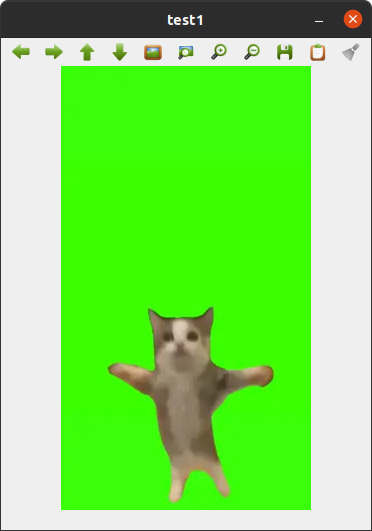
\includegraphics[width=0.2\columnwidth]{image/image1.png}
        \caption{imshow関数の実行結果}
        \label{fig:imshow}
        \end{center}
    \end{figure}

    画像の拡大縮小はresize関数を用いる.resize関数はサイズを直接指定する方法と縦横の倍率を指定する方法がある.
    実際にサイズを直接指定する方法で横を2倍にした画像と縦横の倍率を指定する方法で縦を1/2倍にした画像を図\ref{fig:large1},\ref{fig:large2}
    \begin{figure}[H]
        \begin{center}
        
\includegraphics[width=0.22\columnwidth]{image/result1.png}
        \caption{横を2倍にする}
        \label{fig:large1}
        \end{center}
    \end{figure}
    \begin{figure}[H]
        \begin{center}
        
\includegraphics[width=0.22\columnwidth]{image/result2.png}
        \caption{縦を1/2倍にする} %後で差し替え
        \label{fig:large2}
        \end{center}
    \end{figure}

    \newpage
    画像の回転はrotate関数を用いる.ROTATE\_90\_CLOCKWISE,ROTATE\_90\_COUNTERCLOCKWISE,ROTATE\_180は右に90度,左に90度,180度回転する.
    \begin{figure}[H]
        \begin{tabular}{ccc}
            \begin{minipage}{.33\textwidth}
                \centering
                
\includegraphics[width=0.5\linewidth]{image/result3.png}
                \caption{右に90度回転}
                \label{f1}
            \end{minipage}
            \begin{minipage}{.33\textwidth}
                \centering
                
\includegraphics[width=0.5\linewidth]{image/result4.png}
                \caption{左に90度回転}
                \label{f2}
            \end{minipage}
            \begin{minipage}{.33\textwidth}
                \centering
                
\includegraphics[width=0.5\linewidth]{image/result5.png}
                \caption{180度回転}
                \label{f3}
            \end{minipage}
        \end{tabular}
    \end{figure}
    
    二値化をする画像は以下の図\ref{fig:gray}とする.
    \begin{figure}[H]
        \begin{center}
        
\includegraphics[width=0.1\columnwidth]{image/image2.png}
        \caption{二値化に使用する画像}
        \label{fig:gray}
        \end{center}
    \end{figure}
    二値化はthreshold関数を用いる.閾値を100として超えた場合255に変更した画像が図\ref{fig:scal1},閾値を自動で設定した場合の画像が図\ref{fig:scal2}である.
    \begin{figure}[H]
        \begin{tabular}{cc}
            \begin{minipage}{.5\textwidth}
                \centering
                
\includegraphics[width=0.3\linewidth]{image/result6.png}
                \caption{閾値を100として設定した場合}
                \label{fig:scal1}
            \end{minipage}
            \begin{minipage}{.5\textwidth}
                \centering
                
\includegraphics[width=0.3\linewidth]{image/result7.png}
                \caption{閾値を自動で設定した場合}
                \label{fig:scal2}
            \end{minipage}
        \end{tabular}
    \end{figure}

    \section{画像の特徴量抽出と図示}
    使用する画像として図\ref{fig:tomato},図\ref{fig:sea}を用いる.
    \begin{figure}[H]
        \begin{tabular}{cc}
            \begin{minipage}{.5\textwidth}
                \centering
                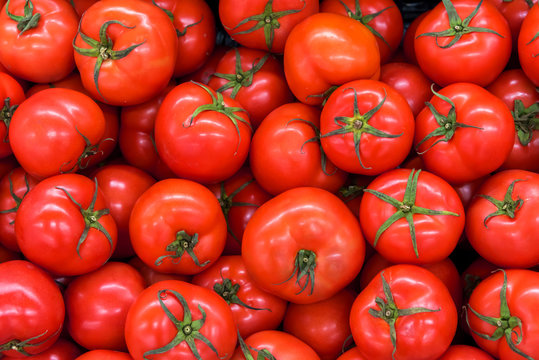
\includegraphics[width=0.5\linewidth]{tomato.png}
                \caption{トマト}
                \label{fig:tomato}
            \end{minipage}
            \begin{minipage}{.5\textwidth}
                \centering
                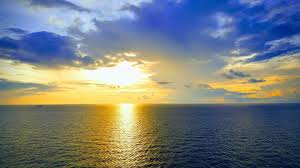
\includegraphics[width=0.5\linewidth]{sea.png}
                \caption{海}
                \label{fig:sea}
            \end{minipage}
        \end{tabular}
    \end{figure}
    
	% \newpage
	% \begin{center}
	% 	{\LARGE \bf 応用課題}
	% \end{center}
	
\end{document}
